% Part 1 - Document Setup and Preamble
\documentclass[11pt,a4paper]{article}
\usepackage[margin=1in]{geometry}
\usepackage{amsmath}
\usepackage{amssymb}
\usepackage{titlesec}
\usepackage{enumitem}
\usepackage{xcolor}
\usepackage[most]{tcolorbox}
\usepackage{fancyhdr}
\usepackage{listings}
\usepackage{hyperref}
\usepackage{graphicx}
\usepackage{tikz}
\usetikzlibrary{shapes.geometric, arrows, positioning, fit, backgrounds}
\usetikzlibrary{calc}

\newcommand{\wrongmark}{\times}
\usepackage[utf8]{inputenc}
\usepackage{newunicodechar}
\newunicodechar{✓}{\checkmark}
\newunicodechar{✗}{\wrongmark}

% Header and Footer
\pagestyle{fancy}
\fancyhf{}
\rhead{Pydantic Complete Guide}
\lhead{Data Validation in Python}
\cfoot{\thepage}

% Title formatting
\titleformat{\section}{\Large\bfseries\color{blue!70!black}}{\thesection}{1em}{}[\titlerule]
\titleformat{\subsection}{\large\bfseries\color{blue!50!black}}{\thesubsection}{1em}{}
\titleformat{\subsubsection}{\normalsize\bfseries\color{blue!40!black}}{\thesubsubsection}{1em}{}

% Code styling
\definecolor{codebg}{gray}{0.95}
\definecolor{codegreen}{rgb}{0,0.6,0}
\definecolor{codegray}{rgb}{0.5,0.5,0.5}
\definecolor{codepurple}{rgb}{0.58,0,0.82}

\lstdefinestyle{pythonstyle}{
    language=Python,
    backgroundcolor=\color{codebg},
    commentstyle=\color{codegreen},
    keywordstyle=\color{blue},
    numberstyle=\tiny\color{codegray},
    stringstyle=\color{codepurple},
    basicstyle=\ttfamily\small,
    breaklines=true,
    captionpos=b,
    keepspaces=true,
    numbers=left,
    numbersep=5pt,
    showspaces=false,
    showstringspaces=false,
    showtabs=false,
    tabsize=4,
    frame=single,
    xleftmargin=2em,
    framexleftmargin=1.5em
}

\lstset{style=pythonstyle}

% Command box
\newtcolorbox{cmdbox}{
    colback=codebg,
    colframe=black!50,
    boxrule=0.5pt,
    left=2mm,
    right=2mm,
    top=1mm,
    bottom=1mm,
    breakable
}

% Example box
\newtcolorbox{examplebox}[1]{
    colback=green!5!white,
    colframe=green!75!black,
    title=#1,
    fonttitle=\bfseries,
    breakable,
    enhanced jigsaw
}

% Note box
\newtcolorbox{notebox}{
    colback=yellow!10!white,
    colframe=orange!75!black,
    title=Important Note,
    fonttitle=\bfseries,
    breakable,
    enhanced jigsaw
}

% Warning box
\newtcolorbox{warningbox}{
    colback=red!5!white,
    colframe=red!75!black,
    title=Warning,
    fonttitle=\bfseries,
    breakable,
    enhanced jigsaw
}

% Info box
\newtcolorbox{infobox}[1]{
    colback=blue!5!white,
    colframe=blue!75!black,
    title=#1,
    fonttitle=\bfseries,
    breakable,
    enhanced jigsaw
}

\begin{document}

% Title Page
\begin{titlepage}
    \centering
    \vspace*{2cm}
    {\Huge\bfseries Pydantic\\[0.5cm] Complete Guide\par}
    \vspace{1cm}
    {\Large Data Validation and Type Safety in Python\par}
    \vspace{2cm}
    {\large A Comprehensive Guide to Pydantic,\\
    Data Models, Validation, and Production-Grade Python Code\par}
    \vspace{3cm}
    {\Large\bfseries Learning Notes\par}
    \vspace{0.5cm}
    {\large Based on Comprehensive Tutorial\par}
    \vspace{3cm}
    {\Large\bfseries Sujil S\par}
    \vspace{0.5cm}
    {\large\texttt{sujil9480@gmail.com}\par}
    \vfill
    {\large \today\par}
\end{titlepage}

\tableofcontents
\newpage

% ========================
% SECTION 1: INTRODUCTION
% ========================
\section{Introduction to Pydantic}

\subsection{What is Pydantic?}

\begin{infobox}{Definition}
\textbf{Pydantic is a powerful Python library for data validation and settings management using Python type annotations.}
\end{infobox}

Pydantic enables you to:
\begin{itemize}[leftmargin=*]
    \item Perform type validation automatically
    \item Validate complex data structures
    \item Build robust data models
    \item Structure complex data easily
    \item Write production-grade code with confidence
\end{itemize}

\subsection{Why Pydantic Matters}

\begin{notebox}
Python is a \textbf{dynamically typed language}, which means it does not have static typing like Java or C++. While this flexibility is great for beginners, it becomes a significant challenge when writing production-grade code.

\vspace{0.5em}
\textbf{The Challenge}: Without proper validation, you cannot ensure:
\begin{itemize}[leftmargin=*]
    \item Variables contain the correct type
    \item Data meets business requirements
    \item Invalid data doesn't enter your system
\end{itemize}
\end{notebox}

\subsection{Where Pydantic is Used}

Pydantic is extensively used across various domains:

\begin{enumerate}[leftmargin=*]
    \item \textbf{FastAPI}: Building REST APIs (Pydantic is core to FastAPI)
    \item \textbf{Configuration Management}: YAML/JSON config file validation
    \item \textbf{Data Science}: ML pipeline data validation
    \item \textbf{Data Engineering}: ETL pipeline data structures
    \item \textbf{Any Production Code}: Where data integrity is critical
\end{enumerate}

\begin{infobox}{Industry Importance}
If you're entering the data science or software engineering industry, having solid knowledge of Pydantic is \textbf{essential}.
\end{infobox}

\newpage

% ========================
% SECTION 2: THE PROBLEMS
% ========================
\section{Understanding the Problems Pydantic Solves}

Before diving into solutions, let's understand exactly what problems Pydantic addresses.

\subsection{Problem Setup: Patient Management System}

Let's consider a real-world scenario where we're building a function to insert patient data into a database.

\subsubsection{The Basic Function}

\begin{lstlisting}[language=Python, caption=Initial Patient Insertion Function]
def insert_patient_data(patient_name, patient_age):
    """
    Insert patient data into database
    """
    print(patient_name)
    print(patient_age)
    
    # Imagine database insertion code here
    return "Patient data inserted successfully"
\end{lstlisting}

\textbf{The Scenario}:
\begin{itemize}[leftmargin=*]
    \item A senior programmer writes this function
    \item A junior programmer will use it to insert data
    \item The junior programmer only sees the function signature
    \item They don't see the implementation details
\end{itemize}

\subsection{Problem 1: No Type Validation}

\subsubsection{What Can Go Wrong}

The junior programmer might do this:

\begin{lstlisting}[language=Python, caption=Problematic Usage]
insert_patient_data("John Doe", "30")  # Age as string!
\end{lstlisting}

\textbf{The Issue}:
\begin{itemize}[leftmargin=*]
    \item We expected \texttt{patient\_age} to be an integer
    \item But the junior programmer sent it as a string
    \item \textbf{The code will still work!}
    \item Wrong data type gets inserted into the database
\end{itemize}

\begin{warningbox}
\textbf{This is a serious failure!}

\vspace{0.5em}
In production databases, you want to enforce a strict schema:
\begin{itemize}[leftmargin=*]
    \item All patient names should be strings
    \item All patient ages should be integers
    \item No exceptions!
\end{itemize}

But our current code doesn't enforce this at all.
\end{warningbox}

\subsubsection{Attempt 1: Type Hints}

Let's try Python's type hinting:

\begin{lstlisting}[language=Python, caption=Adding Type Hints]
def insert_patient_data(patient_name: str, patient_age: int):
    print(patient_name)
    print(patient_age)
    return "Patient data inserted successfully"

# Usage
insert_patient_data("John Doe", 30)  # Correct
\end{lstlisting}

\textbf{Benefits}:
\begin{itemize}[leftmargin=*]
    \item IDE shows suggested types
    \item Documentation is clearer
    \item Other developers see expected types
\end{itemize}

\textbf{Problem}:
\begin{itemize}[leftmargin=*]
    \item Type hints are just \textit{suggestions}
    \item They don't enforce anything
    \item Wrong types still work!
\end{itemize}

\begin{lstlisting}[language=Python, caption=Type Hints Don't Stop This]
# This still works even though age is wrong type!
insert_patient_data("John Doe", "30")  # No error!
\end{lstlisting}

\begin{notebox}
\textbf{Key Understanding}: Python's type hints provide information but do NOT enforce types. The code will execute even with wrong types.
\end{notebox}

\subsubsection{Attempt 2: Manual Validation}

Let's enforce types manually:

\begin{lstlisting}[language=Python, caption=Manual Type Checking]
def insert_patient_data(patient_name: str, patient_age: int):
    
    if type(patient_name) == str and type(patient_age) == int:
        print(patient_name)
        print(patient_age)
        return "Patient data inserted successfully"
    else:
        raise ValueError("Invalid input types")

# Now this will raise an error
insert_patient_data("John Doe", "30")  # ValueError!
\end{lstlisting}

\textbf{This Works!} But is it a good solution?

\vspace{0.5em}
\textit{Note: In real Python code, \texttt{isinstance()} is preferred over
\texttt{type() ==} because it correctly handles inheritance and subclasses.}

\subsubsection{The Scalability Problem}

Consider if you need multiple functions:

\begin{lstlisting}[language=Python, caption=Multiple Functions Need Same Validation]
def insert_patient_data(patient_name: str, patient_age: int):
    if type(patient_name) == str and type(patient_age) == int:
        # Insert logic
        pass
    else:
        raise ValueError("Invalid input")

def update_patient_data(patient_name: str, patient_age: int):
    if type(patient_name) == str and type(patient_age) == int:
        # Update logic
        pass
    else:
        raise ValueError("Invalid input")
\end{lstlisting}

\textbf{Problems}:
\begin{itemize}[leftmargin=*]
    \item Repeating the same validation code
    \item Just 2 fields and 2 functions - already messy
    \item What if you have 10 fields? 20 functions?
    \item What if you add a new field later?
    \item Need to update ALL functions!
\end{itemize}

\begin{warningbox}
\textbf{This approach doesn't scale!}

\vspace{0.5em}
Writing manual validation code for every function is:
\begin{itemize}[leftmargin=*]
    \item Time-consuming
    \item Error-prone
    \item Difficult to maintain
    \item Not DRY (Don't Repeat Yourself)
\end{itemize}
\end{warningbox}

\newpage

\subsection{Problem 2: Data Validation}

Type validation is just the beginning. We also need to validate \textbf{data constraints}.

\subsubsection{Business Rules}

Consider these realistic requirements:

\begin{itemize}[leftmargin=*]
    \item \textbf{Age}: Cannot be negative
    \item \textbf{Email}: Must follow email format
    \item \textbf{Phone}: Must be valid phone format
    \item \textbf{Many more constraints...}
\end{itemize}

\subsubsection{Manual Data Validation}

\begin{lstlisting}[language=Python, caption=Adding Data Validation]
def insert_patient_data(patient_name: str, patient_age: int):
    
    # Type validation
    if type(patient_name) == str and type(patient_age) == int:
        
        # Data validation
        if patient_age < 0:
            raise ValueError("Age cannot be negative")
        else:
            print(patient_name)
            print(patient_age)
            return "Patient data inserted successfully"
    else:
        raise ValueError("Invalid input types")

# This will fail
insert_patient_data("John Doe", -1)  # ValueError: Age cannot be negative
\end{lstlisting}

\textbf{Now we have}:
\begin{itemize}[leftmargin=*]
    \item Type validation (str, int)
    \item Data validation (age $>$ 0)
\end{itemize}

\subsubsection{The Complexity Explosion}

Imagine adding more fields:

\begin{lstlisting}[language=Python, caption=Complexity Grows Quickly]
def insert_patient_data(patient_name: str, 
                       patient_age: int,
                       patient_email: str,
                       patient_phone: str):
    
    # Type validation for all fields
    if (type(patient_name) == str and 
        type(patient_age) == int and
        type(patient_email) == str and
        type(patient_phone) == str):
        
        # Data validation for age
        if patient_age < 0:
            raise ValueError("Age cannot be negative")
        
        # Data validation for email
        # Need regex for email format!
        
        # Data validation for phone
        # Need validation for phone format!
        
        # ... more validations ...
        
        # Finally, insert data
        pass
\end{lstlisting}

\textbf{The Nightmare}:
\begin{itemize}[leftmargin=*]
    \item 10 fields = 10 type checks + 10 data validations
    \item Tons of boilerplate code
    \item Must repeat in EVERY function
    \item Adding a new field = updating ALL functions
    \item Email/phone validation requires regex patterns
\end{itemize}

\begin{warningbox}
\textbf{This is exactly the problem Pydantic solves!}

\vspace{0.5em}
Pydantic ensures:
\begin{itemize}[leftmargin=*]
    \item Automatic type validation
    \item Automatic data validation
    \item No repetitive boilerplate code
    \item Centralized validation logic
    \item Easy to maintain and extend
\end{itemize}
\end{warningbox}

\subsection{Summary: The Two Core Problems}

\begin{center}
\begin{tabular}{|p{0.45\textwidth}|p{0.45\textwidth}|}
\hline
\textbf{Problem 1: Type Validation} & \textbf{Problem 2: Data Validation} \\
\hline
Python is dynamically typed & Data must meet business rules \\
\hline
Type hints don't enforce types & Age cannot be negative \\
\hline
Manual type checking is tedious & Email must be valid format \\
\hline
Not scalable for production code & Phone must be valid format \\
\hline
\multicolumn{2}{|c|}{\textbf{Pydantic solves both problems elegantly}} \\
\hline
\end{tabular}
\end{center}

\newpage

% ========================
% SECTION 3: PYDANTIC SOLUTION
% ========================
\section{The Pydantic Solution}

\subsection{How Pydantic Works: 3-Step Process}

Pydantic follows a clean, three-step workflow:

\begin{center}
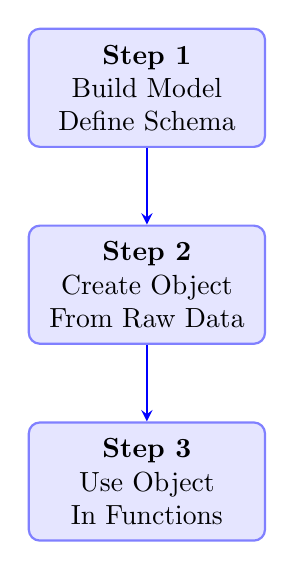
\begin{tikzpicture}[
    node distance=2.5cm,
    procstep/.style={rectangle, rounded corners, draw=blue!50, fill=blue!10, thick, minimum width=3cm, minimum height=1.5cm, align=center},
    arrow/.style={->, >=stealth, thick, blue}
]

\node[procstep] (step1) {\textbf{Step 1}\\Build Model\\Define Schema};
\node[procstep, below of=step1] (step2) {\textbf{Step 2}\\Create Object\\From Raw Data};
\node[procstep, below of=step2] (step3) {\textbf{Step 3}\\Use Object\\In Functions};

\draw[arrow] (step1) -- (step2);
\draw[arrow] (step2) -- (step3);

\end{tikzpicture}
\end{center}

\subsubsection{Step 1: Build a Pydantic Model}

A model is a class that defines your data schema:

\begin{itemize}[leftmargin=*]
    \item Define which fields you need
    \item Specify the data type for each field
    \item Add validation constraints
\end{itemize}

\textbf{Example}: For patient data, you define:
\begin{itemize}[leftmargin=*]
    \item Field: \texttt{name}, Type: \texttt{str}
    \item Field: \texttt{age}, Type: \texttt{int}
    \item Constraint: age should always be $>$ 0
\end{itemize}

\subsubsection{Step 2: Instantiate the Model}

You create an object from the model using raw input data:

\begin{itemize}[leftmargin=*]
    \item Prepare data as a dictionary
    \item Pass it to the Pydantic model
    \item \textbf{Validation happens automatically here!}
\end{itemize}

\textbf{During this step}:
\begin{itemize}[leftmargin=*]
    \item Type validation is performed
    \item Data validation is performed
    \item If all checks pass → you get a validated object
    \item If any check fails → automatic error is raised
\end{itemize}

\subsubsection{Step 3: Use the Validated Object}

Pass the validated Pydantic object to your functions:

\begin{itemize}[leftmargin=*]
    \item Functions receive validated data
    \item No need for manual validation inside functions
    \item Clean, maintainable code
\end{itemize}

\begin{notebox}
\textbf{Key Insight}: Validation happens in Step 2, not in your business logic functions. This separation of concerns makes code much cleaner.
\end{notebox}

\newpage

\subsection{Practical Implementation}

\subsubsection{Installation}

First, install Pydantic:

\begin{cmdbox}
\begin{verbatim}
pip install pydantic
\end{verbatim}
\end{cmdbox}

\begin{infobox}{Pydantic Versions}
\textbf{Use Pydantic V2}

\vspace{0.5em}
Pydantic has two major versions:
\begin{itemize}[leftmargin=*]
    \item V1: Older version
    \item V2: Current version (recommended)
\end{itemize}

\textbf{Why V2?}
\begin{itemize}[leftmargin=*]
    \item Written in Rust (much faster)
    \item Better features and improvements
    \item Industry standard going forward
\end{itemize}

Always ensure you're using Pydantic V2 for new projects.
\end{infobox}

\subsubsection{Step 1: Import and Create Model}

\begin{lstlisting}[language=Python, caption=Creating Your First Pydantic Model]
from pydantic import BaseModel

class Patient(BaseModel):
    patient_name: str
    patient_age: int
\end{lstlisting}

\textbf{What's happening}:
\begin{itemize}[leftmargin=*]
    \item Import \texttt{BaseModel} from pydantic
    \item Create a class that inherits from \texttt{BaseModel}
    \item Define fields with type annotations
\end{itemize}

\begin{notebox}
\textbf{Important}: Your model class MUST inherit from \texttt{BaseModel}. This is what makes it a Pydantic model.
\end{notebox}

\subsubsection{Step 2: Create Validated Object}

\begin{lstlisting}[language=Python, caption=Instantiating the Model]
# Raw data as dictionary
patient_info = {
    'patient_name': "Nitish",
    'patient_age': 30
}

# Create Pydantic object (validation happens here!)
patient_1 = Patient(**patient_info)
\end{lstlisting}

\textbf{Behind the scenes}:
\begin{itemize}[leftmargin=*]
    \item Pydantic checks if \texttt{patient\_name} is a string ✓
    \item Pydantic checks if \texttt{patient\_age} is an integer ✓
    \item All validation passes → object created successfully
\end{itemize}

\subsubsection{Step 3: Use in Functions}

\begin{lstlisting}[language=Python, caption=Using Validated Objects in Functions]
def insert_patient_data(patient: Patient):
    """
    Function now receives validated Patient object
    No manual validation needed!
    """
    print(patient.patient_name)
    print(patient.patient_age)
    return "Patient data inserted successfully"

# Call function with validated object
insert_patient_data(patient_1)
\end{lstlisting}

\textbf{Key observations}:
\begin{itemize}[leftmargin=*]
    \item Function signature specifies \texttt{Patient} type
    \item No manual validation code inside function
    \item Access fields using dot notation: \texttt{patient.patient\_name}
    \item Clean and readable code
\end{itemize}

\subsection{Complete Working Example}

\begin{lstlisting}[language=Python, caption=Full Pydantic Example]
from pydantic import BaseModel

# Step 1: Define Model
class Patient(BaseModel):
    patient_name: str
    patient_age: int

# Step 2: Create Validated Object
patient_info = {'patient_name': "Nitish", 'patient_age': 30}
patient_1 = Patient(**patient_info)

# Step 3: Use in Function
def insert_patient_data(patient: Patient):
    print(patient.patient_name)
    print(patient.patient_age)
    return "Patient data inserted successfully"

insert_patient_data(patient_1)
\end{lstlisting}

\textbf{Output}:
\begin{cmdbox}
\begin{verbatim}
Nitish
30
\end{verbatim}
\end{cmdbox}

\subsection{Automatic Validation in Action}

\subsubsection{What Happens with Wrong Type}

\begin{lstlisting}[language=Python, caption=Invalid Data Example]
# Wrong type for age (string instead of int)
patient_info = {'patient_name': "Nitish", 'patient_age': "thirty"}
patient_1 = Patient(**patient_info)  # This will fail!
\end{lstlisting}

\textbf{Result}:
\begin{cmdbox}
\begin{verbatim}
ValidationError: 
  patient_age
    Input should be a valid integer
\end{verbatim}
\end{cmdbox}

\begin{infobox}{Automatic Error Handling}
Pydantic automatically:
\begin{itemize}[leftmargin=*]
    \item Detects the type mismatch
    \item Raises a descriptive \texttt{ValidationError}
    \item Tells you exactly what's wrong
    \item Prevents invalid data from entering your system
\end{itemize}

All without you writing any validation code!
\end{infobox}

\subsection{Benefits Achieved}

\begin{center}
\begin{tabular}{|p{0.45\textwidth}|p{0.45\textwidth}|}
\hline
\textbf{Before Pydantic} & \textbf{With Pydantic} \\
\hline
Manual type checking in every function & Define schema once \\
\hline
Repetitive validation code & No repetition \\
\hline
Easy to miss validations & Automatic validation \\
\hline
Hard to maintain & Easy to maintain \\
\hline
Difficult to extend & Easy to add new fields \\
\hline
Boilerplate everywhere & Clean, readable code \\
\hline
\end{tabular}
\end{center}

\newpage

\subsection{Type Coercion: Pydantic's Smart Feature}

Pydantic doesn't just validate - it can also intelligently convert types.

\subsubsection{Automatic Type Conversion}

\begin{lstlisting}[language=Python, caption=Pydantic Type Coercion]
# Age as string "30" instead of integer 30
patient_info = {'patient_name': "Nitish", 'patient_age': "30"}
patient_1 = Patient(**patient_info)

# Pydantic converts "30" to 30 automatically!
print(patient_1.patient_age)  # Output: 30 (integer)
\end{lstlisting}

\textbf{What happened}:
\begin{itemize}[leftmargin=*]
    \item You provided age as string \texttt{"30"}
    \item Pydantic detected it should be integer
    \item Pydantic successfully converted it to \texttt{30}
    \item No error raised - smart conversion!
\end{itemize}

\subsubsection{When Coercion Works}

Pydantic performs type coercion when conversion makes sense:

\begin{center}
\begin{tabular}{|l|l|l|}
\hline
\textbf{Input Type} & \textbf{Expected Type} & \textbf{Result} \\
\hline
\texttt{"30"} & \texttt{int} & ✓ Converted to 30 \\
\hline
\texttt{"3.14"} & \texttt{float} & ✓ Converted to 3.14 \\
\hline
\texttt{"true"} & \texttt{bool} & ✓ Converted to True \\
\hline
\texttt{"thirty"} & \texttt{int} & $\wrongmark$ Cannot convert \\
\hline
\end{tabular}
\end{center}

\begin{notebox}
\textbf{Smart, Not Magic}

\vspace{0.5em}
Pydantic coercion is intelligent:
\begin{itemize}[leftmargin=*]
    \item \texttt{"30"} to \texttt{int}: Works ✓
    \item \texttt{"thirty"} to \texttt{int}: Fails $\wrongmark$
    \item Only valid conversions are performed
\end{itemize}
\end{notebox}

\subsection{Multiple Functions: The Real Benefit}

\subsubsection{Before Pydantic}

\begin{lstlisting}[language=Python, caption=Without Pydantic - Repeated Code]
def insert_patient_data(patient_name: str, patient_age: int):
    if type(patient_name) == str and type(patient_age) == int:
        # Logic here
        pass
    else:
        raise ValueError("Invalid input")

def update_patient_data(patient_name: str, patient_age: int):
    if type(patient_name) == str and type(patient_age) == int:
        # Logic here
        pass
    else:
        raise ValueError("Invalid input")

# Repeated validation in every function!
\end{lstlisting}

\subsubsection{With Pydantic}

\begin{lstlisting}[language=Python, caption=With Pydantic - Clean Code]
class Patient(BaseModel):
    patient_name: str
    patient_age: int

def insert_patient_data(patient: Patient):
    # No validation code needed
    pass

def update_patient_data(patient: Patient):
    # No validation code needed
    pass

# Validation defined once, used everywhere!
\end{lstlisting}

\begin{infobox}{Key Advantage}
With Pydantic:
\begin{itemize}[leftmargin=*]
    \item Define validation once in the model
    \item All functions automatically benefit
    \item Adding a new field? Update only the model
    \item Changes propagate to all functions automatically
\end{itemize}
\end{infobox}

\newpage

% ========================
% SECTION 4: BUILDING COMPLEX MODELS
% ========================
\section{Building Complex Pydantic Models}

\subsection{Working with Multiple Data Types}

Let's build a more realistic patient model with various data types.

\subsubsection{Extended Patient Model}

\begin{lstlisting}[language=Python, caption=Complex Patient Model]
from pydantic import BaseModel
from typing import List, Dict, Optional

class Patient(BaseModel):
    name: str
    age: int
    weight: float
    height: float
    bmi: float
    married: bool
    allergies: List[str]
    contact_details: Dict[str, str]
\end{lstlisting}

\textbf{Data types covered}:
\begin{itemize}[leftmargin=*]
    \item \texttt{str}: Text fields (name)
    \item \texttt{int}: Whole numbers (age)
    \item \texttt{float}: Decimal numbers (weight, height, bmi)
    \item \texttt{bool}: True/False values (married)
    \item \texttt{List[str]}: List of strings (allergies)
    \item \texttt{Dict[str, str]}: Dictionary with string keys/values (contact details)
\end{itemize}

\subsection{Why Import from typing Module}

\subsubsection{The Question}

Why do we write \texttt{List[str]} instead of just \texttt{list}?

\begin{lstlisting}[language=Python, caption=Understanding the Difference]
# Wrong way
allergies: list  # Only validates it's a list

# Right way
allergies: List[str]  # Validates it's a list AND items are strings
\end{lstlisting}

\textbf{The difference}:
\begin{itemize}[leftmargin=*]
    \item \texttt{list}: Only checks if variable is a list
    \item \texttt{List[str]}: Checks if it's a list AND every item is a string
\end{itemize}

\subsubsection{Two-Level Validation}

\begin{lstlisting}[language=Python, caption=List Validation Example]
from typing import List

class Patient(BaseModel):
    allergies: List[str]

# Valid
patient_1 = Patient(allergies=["Pollen", "Dust"])  

# Invalid - not a list
patient_2 = Patient(allergies="Pollen")  

# Invalid - list but contains integer
patient_3 = Patient(allergies=["Pollen", 123])  
\end{lstlisting}

\textbf{What Pydantic validates}:
\begin{enumerate}[leftmargin=*]
    \item Is \texttt{allergies} a list? (First level)
    \item Is every item in the list a string? (Second level)
\end{enumerate}

\begin{notebox}
This two-level validation is why we use \texttt{List[str]} from the typing module instead of just \texttt{list}.
\end{notebox}

\subsubsection{Dictionary Validation}

Same concept applies to dictionaries:

\begin{lstlisting}[language=Python, caption=Dictionary Validation]
from typing import Dict

class Patient(BaseModel):
    contact_details: Dict[str, str]

# Valid - keys and values are strings
patient = Patient(
    contact_details={'email': 'abc@gmail.com', 'phone': '9876543210'}
)  

# Invalid - value is integer
patient = Patient(
    contact_details={'phone': 9876543210}
)  
\end{lstlisting}

\textbf{Validation ensures}:
\begin{enumerate}[leftmargin=*]
    \item \texttt{contact\_details} is a dictionary
    \item Every key is a string
    \item Every value is a string
\end{enumerate}

\subsection{Complete Complex Model Example}

\begin{lstlisting}[language=Python, caption=Full Complex Patient Model with Data]
from pydantic import BaseModel
from typing import List, Dict

class Patient(BaseModel):
    name: str
    age: int
    weight: float
    height: float
    bmi: float
    married: bool
    allergies: List[str]
    contact_details: Dict[str, str]

# Create patient with all fields
patient_info = {
    'name': "Sujil S",
    'age': 25,
    'weight': 75.2,
    'height': 175.5,
    'bmi': 24.4,
    'married': True,
    'allergies': ["Pollen", "Dust"],
    'contact_details': {
        'email': 'abc@gmail.com',
        'phone': '9876543210'
    }
}

patient_1 = Patient(**patient_info)

# Access any field
print(patient_1.name)           # Sujil S
print(patient_1.allergies)      # ['Pollen', 'Dust']
print(patient_1.contact_details) # {'email': '...', 'phone': '...'}
\end{lstlisting}

\newpage

% ========================
% SECTION 5: REQUIRED VS OPTIONAL
% ========================
\section{Required and Optional Fields}

\subsection{Default Behavior: All Fields Required}

By default, every field in a Pydantic model is \textbf{required}.

\begin{lstlisting}[language=Python, caption=All Fields Required by Default]
class Patient(BaseModel):
    name: str
    age: int
    weight: float

# Missing 'weight' - will fail!
patient = Patient(name="John", age=30)  # ValidationError!
\end{lstlisting}

\textbf{What happens}:
\begin{itemize}[leftmargin=*]
    \item Pydantic expects ALL fields
    \item If any field is missing → \texttt{ValidationError}
    \item This ensures data completeness
\end{itemize}

\subsection{Making Fields Optional}

Sometimes you want fields that may or may not be provided.

\subsubsection{Using Optional}

\begin{lstlisting}[language=Python, caption=Optional Fields]
from typing import Optional

class Patient(BaseModel):
    name: str              # Required
    age: int               # Required
    allergies: Optional[List[str]] = None  # Optional
\end{lstlisting}

\textbf{What this means}:
\begin{itemize}[leftmargin=*]
    \item \texttt{name} and \texttt{age} are required
    \item \texttt{allergies} is optional
    \item If \texttt{allergies} not provided → defaults to \texttt{None}
\end{itemize}

\begin{notebox}
\textbf{Important Rule}: When you make a field optional, you MUST provide a default value (typically \texttt{None}).
\end{notebox}

\subsubsection{Optional Field Behavior}

\begin{lstlisting}[language=Python, caption=Optional Field Examples]
class Patient(BaseModel):
    name: str
    age: int
    allergies: Optional[List[str]] = None

# Without allergies - works!
patient_1 = Patient(name="John", age=30)
print(patient_1.allergies)  # Output: None

# With allergies - also works!
patient_2 = Patient(
    name="John", 
    age=30, 
    allergies=["Pollen"]
)
print(patient_2.allergies)  # Output: ['Pollen']
\end{lstlisting}

\subsection{Default Values}

You can set default values for any field, not just optional ones.

\subsubsection{Setting Defaults}

\begin{lstlisting}[language=Python, caption=Fields with Default Values]
class Patient(BaseModel):
    name: str                    # Required
    age: int                     # Required
    married: bool = False        # Optional with default
    country: str = "India"       # Optional with default
\end{lstlisting}

\textbf{Behavior}:
\begin{itemize}[leftmargin=*]
    \item If \texttt{married} not provided → defaults to \texttt{False}
    \item If \texttt{country} not provided → defaults to \texttt{"India"}
    \item User can still override defaults
\end{itemize}

\subsubsection{Default Values in Action}

\begin{lstlisting}[language=Python, caption=Using Default Values]
class Patient(BaseModel):
    name: str
    age: int
    married: bool = False

# Not providing 'married'
patient = Patient(name="John", age=30)
print(patient.married)  # Output: False (default value used)

# Explicitly providing 'married'
patient = Patient(name="Jane", age=25, married=True)
print(patient.married)  # Output: True (user value used)
\end{lstlisting}

\subsection{Required vs Optional vs Default: Summary}

\begin{center}
\begin{tabular}{|l|l|l|l|}
\hline
\textbf{Case} & \textbf{Example} & \textbf{Input Required?} & \textbf{Can be None?} \\
\hline
Required & \texttt{name: str} & ✓ Yes & $\wrongmark$ No \\
\hline
Default & \texttt{married: bool = False} & $\wrongmark$ No & $\wrongmark$ No \\
\hline
Required but Nullable & \texttt{x: Optional[int]} & ✓ Yes & ✓ Yes \\
\hline
Optional & \texttt{x: Optional[int] = None} & $\wrongmark$ No & ✓ Yes \\
\hline
\end{tabular}
\end{center}

\begin{notebox}
\textbf{Key Differences (Pydantic v2)}:
\begin{itemize}[leftmargin=*]
    \item \textbf{Required}: Must provide a value, \textbf{cannot be None}
    \item \textbf{Required but Nullable}: Must provide a value, \textbf{can be None} (\texttt{Optional[T]} without default)
    \item \textbf{Default}: Value is optional; if not provided, default is used (cannot be None unless specified)
    \item \textbf{Optional + Default}: Value is optional and \textbf{can be None} (\texttt{Optional[T] = None})
\end{itemize}
\end{notebox}


\newpage

% ========================
% SECTION 6: DATA VALIDATION
% ========================
\section{Data Validation Techniques}

We've covered type validation. Now let's explore data validation - ensuring values meet business rules.

\subsection{Method 1: Custom Data Types}

Pydantic provides specialized types for common validation scenarios.

\subsubsection{EmailStr - Email Validation}

\begin{lstlisting}[language=Python, caption=Email Validation]
from pydantic import BaseModel, EmailStr

class Patient(BaseModel):
    name: str
    email: EmailStr  # Special type for emails

# Valid email
patient = Patient(name="John", email="john@gmail.com")  

# Invalid email (missing @)
patient = Patient(name="John", email="johngmail.com") 
\end{lstlisting}

\textbf{What \texttt{EmailStr} does}:
\begin{itemize}[leftmargin=*]
    \item Validates email format automatically
    \item Checks for \texttt{@} symbol
    \item Ensures proper email structure
    \item No manual validation code needed!
\end{itemize}

\subsubsection{AnyUrl - URL Validation}

\begin{lstlisting}[language=Python, caption=URL Validation]
from pydantic import BaseModel, AnyUrl

class Patient(BaseModel):
    name: str
    linkedin_url: AnyUrl  # Special type for URLs

# Valid URL
patient = Patient(
    name="John",
    linkedin_url="http://linkedin.com/in/john"
)  

# Invalid URL (missing protocol)
patient = Patient(
    name="John",
    linkedin_url="linkedin.com/in/john"
)  
\end{lstlisting}

\textbf{What \texttt{AnyUrl} validates}:
\begin{itemize}[leftmargin=*]
    \item Presence of protocol (http://, https://, etc.)
    \item Valid URL structure
    \item Domain format
\end{itemize}

\begin{notebox}
\textbf{Custom Types Save Time}

\vspace{0.5em}
Manual email/URL validation requires:
\begin{itemize}[leftmargin=*]
    \item Complex regex patterns
    \item Multiple validation checks
    \item Error-prone implementation
\end{itemize}

Pydantic's custom types handle all of this automatically!
\end{notebox}

\subsection{Method 2: Field Function}

For custom business logic validation, use the \texttt{Field} function.

\subsubsection{Importing Field}

\begin{lstlisting}[language=Python, caption=Importing Field and Annotated]
from pydantic import BaseModel, Field
from typing import Annotated
\end{lstlisting}

\subsubsection{Numeric Constraints}

\begin{lstlisting}[language=Python, caption=Validating Numeric Ranges]
class Patient(BaseModel):
    name: str
    age: Annotated[int, Field(gt=0, lt=120)]
    weight: Annotated[float, Field(gt=0)]
\end{lstlisting}

\textbf{Available constraints for numbers}:
\begin{itemize}[leftmargin=*]
    \item \texttt{gt}: Greater than (exclusive)
    \item \texttt{ge}: Greater than or equal
    \item \texttt{lt}: Less than (exclusive)
    \item \texttt{le}: Less than or equal
\end{itemize}

\begin{lstlisting}[language=Python, caption=Testing Numeric Validation]
# Valid age
patient = Patient(name="John", age=25, weight=75.5)  

# Invalid age (negative)
patient = Patient(name="John", age=-5, weight=75.5)  

# Invalid age (too high)
patient = Patient(name="John", age=150, weight=75.5)  
\end{lstlisting}

\subsubsection{String Constraints}

\begin{lstlisting}[language=Python, caption=Validating String Length]
class Patient(BaseModel):
    name: Annotated[str, Field(min_length=3, max_length=50)]
    description: Annotated[str, Field(max_length=200)]
\end{lstlisting}

\textbf{String constraints}:
\begin{itemize}[leftmargin=*]
    \item \texttt{min\_length}: Minimum number of characters
    \item \texttt{max\_length}: Maximum number of characters
\end{itemize}

\begin{lstlisting}[language=Python, caption=Testing String Validation]
# Valid name
patient = Patient(name="John Doe")  

# Invalid - too short
patient = Patient(name="Jo")  

# Invalid - too long (>50 chars)
patient = Patient(
    name="A" * 60
)  
\end{lstlisting}

\subsubsection{List Constraints}

\begin{lstlisting}[language=Python, caption=Validating List Length]
class Patient(BaseModel):
    allergies: Annotated[List[str], Field(max_length=5)]
\end{lstlisting}

\textbf{This ensures}:
\begin{itemize}[leftmargin=*]
    \item Maximum 5 items in the list
    \item Each item must be a string
\end{itemize}

\subsection{Field Function: Multiple Purposes}

The \texttt{Field} function serves three main purposes:

\begin{enumerate}[leftmargin=*]
    \item \textbf{Validation Constraints}: \texttt{gt}, \texttt{lt}, \texttt{min\_length}, etc.
    \item \textbf{Metadata}: Title, description, examples
    \item \textbf{Default Values}: Set defaults directly
    \item \textbf{Type Coercion Control}: Strict mode settings
\end{enumerate}

\subsubsection{Adding Metadata}

\begin{lstlisting}[language=Python, caption=Field with Metadata]
from typing import Annotated

class Patient(BaseModel):
    name: Annotated[
        str,
        Field(
            min_length=3,
            max_length=50,
            title="Patient Name",
            description="Full name of the patient",
            examples=["John Doe", "Jane Smith"]
        )
    ]
\end{lstlisting}

\textbf{Metadata benefits}:
\begin{itemize}[leftmargin=*]
    \item Appears in API documentation (FastAPI)
    \item Helps other developers understand fields
    \item Provides examples for API consumers
    \item Auto-generated documentation uses this
\end{itemize}

\subsubsection{Controlling Type Coercion with Strict Mode}

By default, Pydantic performs type coercion. You can disable this with \texttt{strict=True}.

\begin{lstlisting}[language=Python, caption=Strict Mode Example]
class Patient(BaseModel):
    age: Annotated[int, Field(strict=True)]  # No coercion
    weight: Annotated[float, Field(strict=True)]

# This will fail now
patient = Patient(age="30", weight="75.5")  # ValidationError!

# This works
patient = Patient(age=30, weight=75.5)  # Success
\end{lstlisting}

\textbf{When to use strict mode}:
\begin{itemize}[leftmargin=*]
    \item When exact type matching is critical
    \item In financial applications (no implicit conversions)
    \item When debugging type-related issues
    \item For APIs with strict input requirements
\end{itemize}

\begin{warningbox}
\textbf{Strict Mode Trade-offs}

\vspace{0.5em}
\textbf{Pros}:
\begin{itemize}[leftmargin=*]
    \item Explicit type requirements
    \item Prevents unexpected conversions
    \item Better error detection
\end{itemize}

\textbf{Cons}:
\begin{itemize}[leftmargin=*]
    \item Less forgiving for users
    \item Requires exact type matching
    \item May break existing code
\end{itemize}

\textbf{Strict mode applies per field, not globally (unless using model\_config).}

\vspace{0.3em}
\begin{lstlisting}[language=Python]
from pydantic import ConfigDict

class Patient(BaseModel):
    model_config = ConfigDict(strict=True)
\end{lstlisting}

\end{warningbox}

\newpage

% ========================
% SECTION 7: FIELD VALIDATORS
% ========================
\section{Field Validators: Custom Validation Logic}

\subsection{When to Use Field Validators}

Custom data types and Field constraints cover common cases. But what about business-specific validation?

\vspace{0.5em}
\textbf{Example Scenario}: Hospital tied to specific banks (HDFC, ICICI). Need to validate employee emails from these domains only.

\subsection{Creating Field Validators}

\begin{lstlisting}[language=Python, caption=Email Domain Validation]
from pydantic import BaseModel, field_validator

class Patient(BaseModel):
    name: str
    email: str
    
    @field_validator('email', mode='before')
    @classmethod
    def validate_email_domain(cls, email):
        valid_domains = ['hdfc.com', 'icici.com']
		if '@' not in email:
		    raise ValueError("Invalid email format")

        domain = email.split('@')[1]
        
        if domain not in valid_domains:
            raise ValueError('Invalid domain')
        
        return email
\end{lstlisting}

\subsection{Field Validator Components}

\begin{itemize}[leftmargin=*]
    \item \texttt{@field\_validator('email')}: Specify which field
    \item \texttt{mode='before'/'after'}: When to run
    \item \texttt{@classmethod}: Must be class method
    \item \texttt{cls}: Class reference
    \item \texttt{email}: Field value to validate
\end{itemize}

\subsection{Mode: Before vs After}

\begin{center}
\begin{tabular}{|l|p{0.4\textwidth}|p{0.4\textwidth}|}
\hline
\textbf{Mode} & \textbf{When Runs} & \textbf{Use Case} \\
\hline
\texttt{before} & Before type coercion & Work with raw input \\
\hline
\texttt{after} & After type coercion & Work with converted types \\
\hline
\end{tabular}
\end{center}

\subsection{Transformation with Validators}

\begin{lstlisting}[language=Python, caption=Transform Name to Title Case]
class Patient(BaseModel):
    name: str
    
    @field_validator('name', mode='before')
    @classmethod
    def transform_name(cls, name):
        return name.title()  # Capitalize properly
\end{lstlisting}

\newpage

% ========================
% SECTION 8: MODEL VALIDATORS
% ========================
\section{Model Validators: Cross-Field Validation}

\subsection{The Need for Model Validators}

Field validators work on single fields. What if validation depends on multiple fields?

\vspace{0.5em}
\textbf{Example}: If patient age $>$ 60, emergency contact is required.

\subsection{Creating Model Validators}

\begin{lstlisting}[language=Python, caption=Multi-Field Validation]
from pydantic import model_validator

class Patient(BaseModel):
    age: int
    contact_details: Dict[str, str]
    
    @model_validator(mode='after')
    def validate_emergency_contact(self):
        if self.age > 60:
            if 'emergency' not in self.contact_details:
                raise ValueError(
                    'Patients over 60 need emergency contact'
                )
        return self
\end{lstlisting}

\subsection{Key Differences}

\begin{center}
\begin{tabular}{|l|l|l|}
\hline
\textbf{Aspect} & \textbf{Field Validator} & \textbf{Model Validator} \\
\hline
Scope & Single field & Entire model \\
\hline
Input & Field value & Whole model (self) \\
\hline
Access & One field only & All fields \\
\hline
Return & Field value & Model instance \\
\hline
\end{tabular}
\end{center}

\subsection{Model Validator Modes}

Model validators support three modes: \texttt{before}, \texttt{after}, and \texttt{wrap}.

\subsubsection{Before Mode}

\begin{lstlisting}[language=Python, caption=Before Mode Validator]
class Patient(BaseModel):
    name: str
    age: int
    
    @model_validator(mode='before')
    @classmethod
    def check_data_format(cls, data):
        # data is raw dictionary before any parsing
        if 'age' in data and data['age'] < 0:
            raise ValueError('Age cannot be negative')
        return data
\end{lstlisting}

\textbf{When it runs}: Before Pydantic processes any fields

\subsubsection{After Mode}

\begin{lstlisting}[language=Python, caption=After Mode Validator]
class Patient(BaseModel):
    age: int
    weight: float
    
    @model_validator(mode='after')
    def validate_health_metrics(self):
        # self has all validated fields
        if self.age < 18 and self.weight > 100:
            raise ValueError('Unusual weight for age')
        return self
\end{lstlisting}

\textbf{When it runs}: After all fields are validated and parsed

\subsubsection{Wrap Mode: Advanced Control}

Wrap mode is the most powerful - it lets you control the entire validation process.

\begin{lstlisting}[language=Python, caption=Wrap Mode for Logging]
from typing import Any

class Patient(BaseModel):
    name: str
    email: str
    age: int
    
    @model_validator(mode='wrap')
    @classmethod
    def audit_validation(cls, data: Any, handler):
        try:
            print("Validation starting...")
            # Let Pydantic do its validation
            result = handler(data)
            print("Validation successful!")
            return result
        except ValidationError as e:
            # Log failed validation attempts
            print(f"Validation failed: {e.errors()}")
            print(f"Raw data: {data}")
            raise
\end{lstlisting}

\begin{infobox}{Wrap Mode Use Cases}
\textbf{When to use wrap validators}:
\begin{itemize}[leftmargin=*]
    \item Logging all validation attempts (success/failure)
    \item Audit trails for compliance (HIPAA, GDPR)
    \item Custom retry logic on validation failure
    \item Performance monitoring
    \item Security logging (track invalid inputs)
\end{itemize}
\end{infobox}

\subsection{Understanding Wrap Mode Execution Flow}

\begin{center}
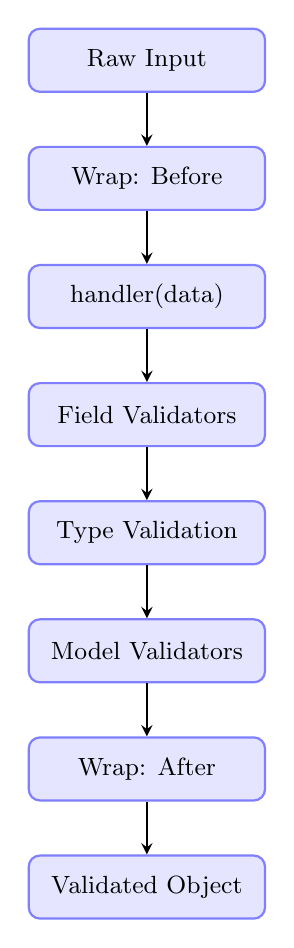
\begin{tikzpicture}[
    node distance=1.5cm,
    process/.style={rectangle, rounded corners, draw=blue!50, fill=blue!10, thick, minimum width=3cm, minimum height=0.8cm, font=\small, align=center},
    arrow/.style={->, >=stealth, thick}
]

\node[process] (input) {Raw Input};
\node[process, below of=input] (wrap1) {Wrap: Before};
\node[process, below of=wrap1] (handler) {handler(data)};
\node[process, below of=handler] (fieldval) {Field Validators};
\node[process, below of=fieldval] (typeval) {Type Validation};
\node[process, below of=typeval] (modelval) {Model Validators};
\node[process, below of=modelval] (wrap2) {Wrap: After};
\node[process, below of=wrap2] (output) {Validated Object};

\draw[arrow] (input) -- (wrap1);
\draw[arrow] (wrap1) -- (handler);
\draw[arrow] (handler) -- (fieldval);
\draw[arrow] (fieldval) -- (typeval);
\draw[arrow] (typeval) -- (modelval);
\draw[arrow] (modelval) -- (wrap2);
\draw[arrow] (wrap2) -- (output);

\end{tikzpicture}
\end{center}

\subsection{Important Limitation: Core Type Parsing}

\begin{warningbox}
\textbf{Important Limitation of Wrap Validators}

\vspace{0.5em}
Wrap validators \textbf{do execute}, but Pydantic’s core type validation
(for types like \texttt{EmailStr} and \texttt{AnyUrl})
happens \textbf{inside} the \texttt{handler(data)} call.

\vspace{0.5em}
This means:
\begin{itemize}[leftmargin=*]
    \item You \textbf{can catch and log} validation errors
    \item You \textbf{cannot intercept or bypass} core type validation
    \item Core type parsing always occurs when \texttt{handler(data)} is invoked
\end{itemize}

\vspace{0.5em}
\begin{lstlisting}[language=Python, caption=Wrap Validator Behavior]
class Patient(BaseModel):
    email: EmailStr
    
    @model_validator(mode='wrap')
    @classmethod
    def log_validation(cls, data, handler):
        try:
            return handler(data)  # Core validation happens here
        except Exception as e:
            print("Caught validation error:", e)
            raise

# Invalid email format (missing @)
patient = Patient(email="invalid")
# Error occurs inside handler(data), not before wrap runs
\end{lstlisting}
\end{warningbox}

\begin{notebox}
\textbf{What is \texttt{handler} in a Wrap Validator?}

\vspace{0.5em}
In a \texttt{@model\_validator(mode="wrap")}, the \texttt{handler} is a
\textbf{callable provided by Pydantic that executes the entire built-in validation pipeline}.

\vspace{0.5em}
Calling \texttt{handler(data)} triggers:
\begin{itemize}[leftmargin=*]
    \item Core type parsing and coercion
    \item Validation of custom types (\texttt{EmailStr}, \texttt{AnyUrl}, etc.)
    \item Field validation and field validators
    \item Model validation (\texttt{before} and \texttt{after})
    \item Construction of the final model instance
\end{itemize}

\vspace{0.5em}
\textbf{Important Rules}:
\begin{itemize}[leftmargin=*]
    \item You \textbf{must call} \texttt{handler(data)} to continue validation
    \item If you do not call it, \textbf{no validation happens}
    \item Any exception raised inside \texttt{handler(data)} represents a validation failure
\end{itemize}

\vspace{0.5em}
\textbf{Key Insight}:
Wrap validators allow you to \textbf{observe, log, or wrap} Pydantic’s validation process,
but they \textbf{do not replace or bypass} core validation logic.
\end{notebox}

\begin{infobox}

\textbf{Final Conclusion}: Why Use \texttt{wrap} Validators?

\vspace{0.5em}
Using a \texttt{wrap} validator does \textbf{not change the validation result}.
The same model is created or the same error is raised whether \texttt{wrap} is used or not.

\vspace{0.5em}
The \textbf{only purpose} of \texttt{wrap} is to \textbf{guarantee observability}
(logging, auditing, monitoring) of the validation process in a centralized way.

\vspace{0.5em}
\textbf{Without \texttt{wrap}}:
\begin{itemize}[leftmargin=*]
    \item Validation still works correctly
    \item Errors can be printed using \texttt{try/except}
    \item Logging must be written manually at every call site
    \item Easy to forget or skip in large codebases
\end{itemize}

\vspace{0.3em}
\textbf{With \texttt{wrap}}:
\begin{itemize}[leftmargin=*]
    \item Validation logic remains exactly the same
    \item Logging is executed automatically for every validation
    \item Observability is enforced at the model level
    \item Cannot be bypassed accidentally
\end{itemize}

\vspace{0.8em}
\textbf{Comparison: With vs Without \texttt{wrap}}

\begin{center}
\begin{tabular}{|p{0.45\textwidth}|p{0.4\textwidth}|}
\hline
\textbf{Without \texttt{wrap}} & \textbf{With \texttt{wrap}} \\
\hline
Validation works correctly & Validation works correctly \\
\hline
Errors can be printed using \texttt{try/except} & Errors can be logged inside the model \\
\hline
Logging must be written manually at every call site & Logging is executed automatically \\
\hline
Easy to forget or skip in large codebases & Enforced for every validation \\
\hline
Responsibility of individual developers & Centralized at model level \\
\hline
Same final result (model or error) & Same final result (model or error) \\
\hline
\end{tabular}
\end{center}

\vspace{0.5em}
\textbf{Correct Example Demonstrating This Behavior}:
\begin{lstlisting}[language=Python]
from pydantic import BaseModel, ValidationError, model_validator

class Patient(BaseModel):
    age: int

    @model_validator(mode="wrap")
    @classmethod
    def audit_validation(cls, data, handler):
        print("AUDIT -> Incoming data:", data)
        try:
            return handler(data)  # Core validation (unchanged)
        except Exception as e:
            print("AUDIT -> Validation failed:", e)
            raise

# Result is the same with or without wrap
try:
    Patient(age="abc")
except ValidationError:
    pass
\end{lstlisting}

\vspace{0.5em}
\textbf{Key Insight}:
Printing errors outside the model and using \texttt{wrap} may produce the same output,
but \texttt{wrap} guarantees that logging and auditing happen \textbf{everywhere and every time},
without relying on individual developers.

\vspace{0.5em}
\textbf{Final Takeaway}:
\texttt{wrap} validators exist for \textbf{enforced observability}, not for validation logic.
\end{infobox}

\newpage

% ========================
% SECTION 9: COMPUTED FIELDS
% ========================
\section{Computed Fields}

\subsection{What are Computed Fields?}

Fields whose values are calculated from other fields, not provided by user.

\vspace{0.5em}
\textbf{Example}: Calculate BMI from weight and height.

\subsection{Implementation}

\begin{lstlisting}[language=Python, caption=Computed BMI Field]
from pydantic import computed_field

class Patient(BaseModel):
    weight: float  # kg
    height: float  # cm
    
    @computed_field
    @property
    def bmi(self) -> float:
        return round(self.weight / (self.height/100)**2, 2)
\end{lstlisting}

\textbf{Key requirements}:
\begin{itemize}[leftmargin=*]
    \item Use \texttt{@computed\_field} decorator
    \item Use \texttt{@property} decorator
    \item Specify return type annotation
    \item Calculate from existing fields
\end{itemize}

\subsection{Usage}

\begin{lstlisting}[language=Python, caption=Using Computed Field]
patient = Patient(weight=75, height=175)
print(patient.bmi)  # Output: 24.49 (automatically calculated)
\end{lstlisting}

\begin{notebox}
\begin{itemize}[leftmargin=*]
    \item Computed fields are read-only and cannot be set by user input.
\end{itemize}
\end{notebox}

\newpage

% ========================
% SECTION 10: NESTED MODELS
% ========================
\section{Nested Models}

\subsection{Why Nested Models?}

Complex data with hierarchical structure needs organization.

\vspace{0.5em}
\textbf{Problem}: Address is complex (city, state, pincode) - storing as string is messy.

\subsection{Creating Nested Models}

\begin{lstlisting}[language=Python, caption=Address as Nested Model]
class Address(BaseModel):
    city: str
    state: str
    pincode: int

class Patient(BaseModel):
    name: str
    age: int
    address: Address  # Nested model as field type
\end{lstlisting}

\subsection{Using Nested Models}

\begin{lstlisting}[language=Python, caption=Creating Nested Objects]
# Create address object
address_info = {'city': 'Bangalore', 'state': 'Karnataka', 'pincode': 560001}
address_1 = Address(**address_info)

# Create patient with nested address
patient_info = {
    'name': 'John',
    'age': 30,
    'address': address_1
}
patient_1 = Patient(**patient_info)

# Access nested fields
print(patient_1.address.city)     # Bangalore
print(patient_1.address.pincode)  # 560001
\end{lstlisting}

\subsection{Benefits}

\begin{enumerate}[leftmargin=*]
    \item \textbf{Organization}: Structured hierarchy
    \item \textbf{Reusability}: Use Address in multiple models
    \item \textbf{Validation}: Automatic validation of nested data
    \item \textbf{Readability}: Clear data structure
\end{enumerate}

\newpage

% ========================
% SECTION 11: EXPORTING DATA
% ========================
\section{Exporting Pydantic Models}

\subsection{Model to Dictionary}

\begin{lstlisting}[language=Python, caption=Export as Dictionary]
patient = Patient(name="John", age=30)

# Export to dict
data = patient.model_dump()
print(data)  # {'name': 'John', 'age': 30}
print(type(data))  # <class 'dict'>
\end{lstlisting}

\subsection{Model to JSON}

\begin{lstlisting}[language=Python, caption=Export as JSON]
json_data = patient.model_dump_json()
print(json_data)  # '{"name":"John","age":30}'
print(type(json_data))  # <class 'str'>
\end{lstlisting}

\subsection{Selective Export}

\begin{lstlisting}[language=Python, caption=Include/Exclude Fields]
# Include only specific fields
data = patient.model_dump(include={'name', 'age'})

# Exclude specific fields
data = patient.model_dump(exclude={'email'})

# Exclude nested fields
data = patient.model_dump(
    exclude={'address': ['state'], 'contact': ['phone']}
)

# Exclude fields with default values not explicitly set
data = patient.model_dump(exclude_unset=True)
\end{lstlisting}

\newpage

% ========================
% SECTION 12: SUMMARY
% ========================
\section{Summary and Best Practices}

\subsection{Key Concepts Covered}

\begin{enumerate}[leftmargin=*]
    \item \textbf{Problem Understanding}: Type and data validation in Python
    \item \textbf{Basic Models}: Creating Pydantic models with BaseModel
    \item \textbf{Data Types}: Working with complex types (List, Dict, Optional)
    \item \textbf{Required/Optional}: Managing field requirements
    \item \textbf{Custom Types}: EmailStr, AnyUrl for common validation
    \item \textbf{Field Function}: Constraints and metadata
    \item \textbf{Field Validators}: Custom single-field validation
    \item \textbf{Model Validators}: Cross-field validation logic
    \item \textbf{Computed Fields}: Calculated fields from other fields
    \item \textbf{Nested Models}: Hierarchical data structures
    \item \textbf{Export Options}: Dictionary and JSON conversion
\end{enumerate}

\subsection{Validation Hierarchy}

\begin{center}
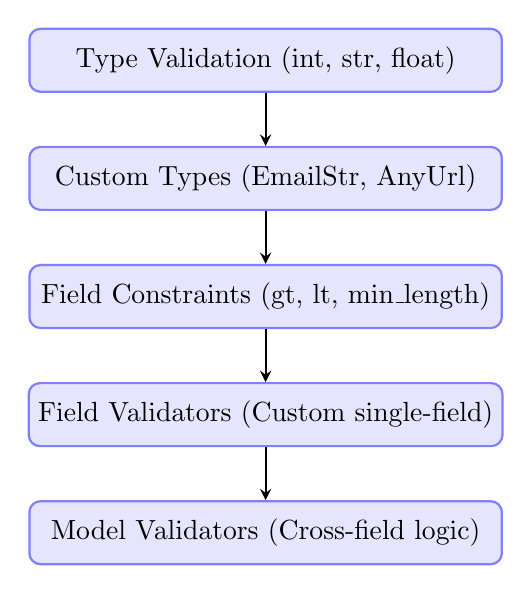
\begin{tikzpicture}[
    node distance=1.5cm,
    level/.style={rectangle, rounded corners, draw=blue!50, fill=blue!10, thick, minimum width=6cm, minimum height=0.8cm, align=center},
    arrow/.style={->, >=stealth, thick}
]

\node[level] (type) {Type Validation (int, str, float)};
\node[level, below of=type] (custom) {Custom Types (EmailStr, AnyUrl)};
\node[level, below of=custom] (field) {Field Constraints (gt, lt, min\_length)};
\node[level, below of=field] (fv) {Field Validators (Custom single-field)};
\node[level, below of=fv] (mv) {Model Validators (Cross-field logic)};

\draw[arrow] (type) -- (custom);
\draw[arrow] (custom) -- (field);
\draw[arrow] (field) -- (fv);
\draw[arrow] (fv) -- (mv);

\end{tikzpicture}
\end{center}

\subsection{Best Practices}

\begin{itemize}[leftmargin=*]
    \item Use Pydantic V2 for new projects
    \item Define clear, descriptive field names
    \item Add metadata for API documentation
    \item Use computed fields for derived values
    \item Nest models for complex hierarchies
    \item Leverage custom types (EmailStr, AnyUrl)
    \item Write field validators for business logic
    \item Use model validators for cross-field rules
\end{itemize}

\subsection{Common Use Cases}

\begin{center}
\begin{tabular}{|l|p{0.6\textwidth}|}
\hline
\textbf{Use Case} & \textbf{Pydantic Feature} \\
\hline
API request/response & BaseModel with Field metadata \\
\hline
Configuration files & Models with default values \\
\hline
Database models & Models with validation \\
\hline
Data pipelines & Computed fields, validators \\
\hline
Complex schemas & Nested models \\
\hline
\end{tabular}
\end{center}

\subsection{Further Learning}

This guide covers beginner to intermediate Pydantic usage. You now have enough knowledge to:

\begin{itemize}[leftmargin=*]
    \item Build FastAPI applications
    \item Validate configuration files
    \item Structure ML pipelines
    \item Write production-grade Python code
\end{itemize}

\begin{infobox}{Next Steps}
Practice by:
\begin{itemize}[leftmargin=*]
    \item Building a simple FastAPI application
    \item Creating models for your domain
    \item Experimenting with complex validators
    \item Exploring Pydantic's official documentation
\end{itemize}
\end{infobox}

\vfill

\begin{center}
\textit{End of Pydantic Complete Guide}

\vspace{1em}

\textit{"Data validation is not just about catching errors—}\\
\textit{it's about building systems you can trust."}

\vspace{1em}

\textbf{Happy coding with Pydantic!}
\end{center}

\end{document}